%----------------------------------------------------------------------------------------
%
% A LaTeX-template for 1DV510. Modified and translated by Björn Lindenberg at LNU.
% Based on an original master thesis template created by Marcus Wilhelmsson at LNU.
%
%----------------------------------------------------------------------------------------

% Settings and document configuration

\documentclass[a4paper,12pt]{article} 
\usepackage[T1]{fontenc} 
\usepackage{times} 
\usepackage[swedish,english]{babel} 
\usepackage[utf8]{inputenc} 
\usepackage{dtk-logos} 
\usepackage{wallpaper} 
\usepackage[absolute]{textpos} 
\usepackage[top=2cm, bottom=2.5cm, left=3cm, right=3cm]{geometry} 
\usepackage[parfill]{parskip} 
\usepackage{csquotes} 
\usepackage{float} 
\usepackage{lipsum} % Used for dummy text. Can be removed.
\usepackage{listings, color}

\lstdefinestyle{Asm}{
  belowcaptionskip=1\baselineskip,
  breaklines=true,
  frame=L,
  xleftmargin=\parindent,
  language=[x86masm]Assembler,
  showstringspaces=false,
  basicstyle=\footnotesize\ttfamily,
  keywordstyle=\bfseries\color{purple!40!black},
  commentstyle=\itshape\color{green!40!black},
  identifierstyle=\color{blue},
  stringstyle=\color{orange},
}

% Fontsizes for section headings.
\usepackage{sectsty} 
\sectionfont{\fontsize{14}{15}\selectfont}
\subsectionfont{\fontsize{12}{15}\selectfont}
\subsubsectionfont{\fontsize{12}{15}\selectfont}

%----------------------------------------------------------------------------------------
%	This part is used for the text box on the title page
%----------------------------------------------------------------------------------------
\newsavebox{\mybox}
\newlength{\mydepth}
\newlength{\myheight}

\newenvironment{sidebar}%
{\begin{lrbox}{\mybox}\begin{minipage}{\textwidth}}%
{\end{minipage}\end{lrbox}%
 \settodepth{\mydepth}{\usebox{\mybox}}%
 \settoheight{\myheight}{\usebox{\mybox}}%
 \addtolength{\myheight}{\mydepth}%
 \noindent\makebox[0pt]{\hspace{-20pt}\rule[-\mydepth]{1pt}{\myheight}}%
 \usebox{\mybox}}

%----------------------------------------------------------------------------------------
%	Title
%----------------------------------------------------------------------------------------
\newcommand\BackgroundPic{
    \put(-2,-3){
    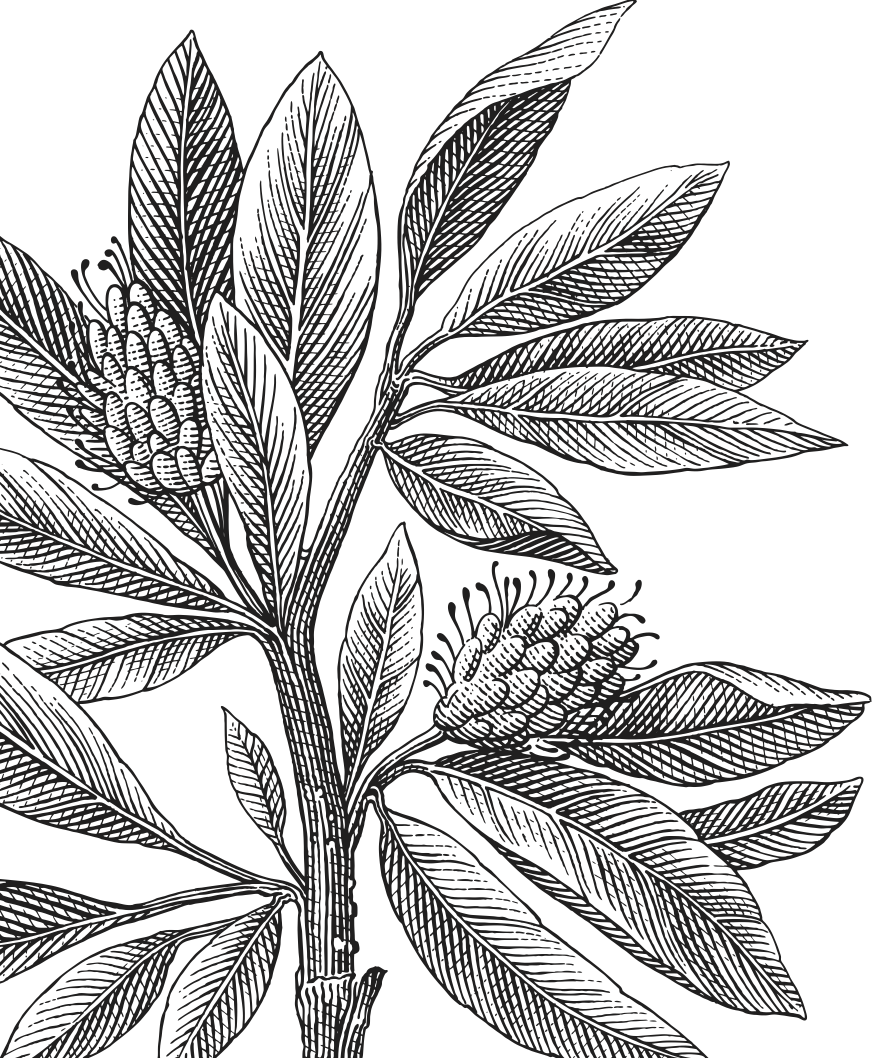
\includegraphics[keepaspectratio,scale=0.3]{img/lnu_etch.png} % Background image
    }
}
\newcommand\BackgroundPicLogo{
    \put(30,740){
    
\includegraphics[keepaspectratio,scale=0.10]{img/logo.png} % LNU logo
    }
}

\title{
\vspace{-8cm}
\begin{sidebar}
    \vspace{10cm}
    \normalfont \normalsize
    \huge Computer Technology I\\ % Main title
    \vspace{-1.3cm}
\end{sidebar}
\vspace{3cm}
\begin{flushleft}
    \huge Lab. 2 : Subroutines % Subtitle
     \small \\ \emph{}
\end{flushleft}
\null
\vfill
\begin{textblock}{5}(10,13)
\begin{flushright}
\begin{minipage}{\textwidth}
\begin{flushleft} \large
\emph{Author:}\textsc{ Loic GALLAND, Leonardo PEDRO}\\  % Author
\emph{Supervisor:}  \textsc{} \\  % Author
\emph{Semester:} Autumn 2019\\ % Semester
\emph{Area:} Computer Science \\ % Area
\emph{Course code:} 1DT301 % Course
\end{flushleft}
\end{minipage}
\end{flushright}
\end{textblock}
}

\date{} % Empty date command. Use \today inside for today's date.
\author{} % Normally one would use this to define authors. However in this case the title command takes care of everything, so we leave the field empty to get rid of warnings. 

\begin{document}

\pagenumbering{gobble} % Turn off page numbering
\newgeometry{left=5cm}
\AddToShipoutPicture*{\BackgroundPic} % Adds the background image to the title page
\AddToShipoutPicture*{\BackgroundPicLogo} % Adds the logo to the title page
\maketitle % Prints the title
\restoregeometry
\clearpage

\pagenumbering{roman} % Roman page numbering for abstract page


\selectlanguage{english}

\newpage

\pagenumbering{gobble} % Turn off page numbering
\tableofcontents 

\newpage
\pagenumbering{arabic} % Turn on page numbering


\section{Task 1 - Switch – Ring counter / Johnson counter}

\textit{Write a program which switch between Ring counter and Johnson counter. You should not use
Interrupt in this lab. The pushbutton must be checked frequently, so there is no delay between the
button is pressed and the change between Ring/Johnson. Use SW0 (PA0) for the button. Each
time you press the button, the program should change counter.}

\lstset{style=Asm}
\begin{lstlisting}
;>>>>>>>>>>>>>>>>>>>>>>>>>>>>>>>>>>>>>>>>>>>>>>>>>>>>>>>>>>>
; 1DT301, Computer Technology I
; Date: 2016-09-15
; Author:
; Loic GALLAND
; Leonardo PEDRO
;
; Lab number: 2
; Title: Subroutines
;
; Hardware: STK600, CPU ATmega2560
;
; Function: Describe the function of the program, so that you can understand it,
; even if you're viewing this in a year from now!
;
; Input ports: Describe the function of used ports, for example on-board switches
; connected to PORTA.
;
; Output ports: Describe the function of used ports, for example on-board LEDs
; connected to PORTB.
;
; Subroutines: If applicable.
; Included files: m2560def.inc
;
; Changes in program: (Description and date)
;<<<<<<<<<<<<<<<<<<<<<<<<<<<<<<<<<<<<<<<<<<<<<<<<<<<<<<<<<<<

.includes "m2560def.inc"
; Initialize SP, Stack Pointer
ldi r20, HIGH(RAMEND) ; R20 = high part of RAMEND address
out SPH,R20 ; SPH = high part of RAMEND address
ldi R20, low(RAMEND) ; R20 = low part of RAMEND address
out SPL,R20 ; SPL = low part of RAMEND address


ldi r16, 0xFF ;setting up the data direction register port B
out DDRB, r16 ;Set port B as output
ldi r16, 0x00
out DDRA, r16

ldi r24, 0b11111110
;ldi r25, 0b11111110

RC:
	ldi r21, 0b11111111; inital LED state
	out portB, r21
	mov r17, r21
	ldi r22, 0xFF
	ldi r23, 0b11111110
 
	RC_loop:
		out portB, r17
		rol r17
		CALL Delay1
		in r25, PINA
		cp r25,r24
		breq JC
		cp r17, r22
		breq RC_light
	rjmp RC_loop
	RC_light:
		rol r17
		out portB, r17
		rjmp RC_loop
rjmp RC

JC:
	ldi r21, 0b11111110
	ldi r22, 0b11111111 ;desired one 
	ldi r23, 0b00000000

	my_loop1:
		out portB, r21
		LSL r21
		CALL Delay1
		in r25, PINA
		cp r25,r24
		breq RC
		cp r21, r23 ;compare  info with desired one 
		breq light
	rjmp my_loop1

	light:
		out portB, r23
		CALL Delay1
		ldi r21, 0b10000000
		out portB, r21
		Second_loop:
			in r25, PINA
			cp r25,r24
			breq RC
			out portB, r21
			ASR r21
			CALL Delay1
			cp r21, r22 ;compare  info with desired one 
			breq my_loop
		rjmp Second_loop
rjmp JC

Delay1:
; Generated by delay loop calculator
; at http://www.bretmulvey.com/avrdelay.html
; Delay 1 950 500 cycles
; 500ms at 3.901 MHz

    ldi  r18, 10
    ldi  r19, 230
    ldi  r20, 22
L1: dec  r20
    brne L1
    dec  r19
    brne L1
    dec  r18
    brne L1
RET
\end{lstlisting}

\newpage
This is the flowchart of the task 1:
\begin{center}
%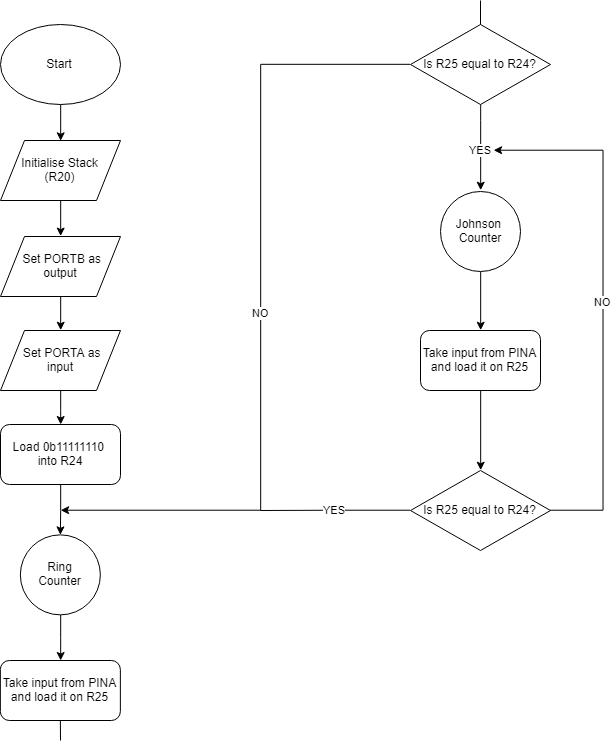
\includegraphics{img/Task1.png}
\end{center}

\section{Task 2 - Electronic dice}
\textit{You should create an electronic dice. Think of the LEDs placed as in the picture below. The
number 1 to 6 should be generated randomly. You could use the fact that the time you press the
button varies in length.}

\lstset{style=Asm}
\begin{lstlisting}
;>>>>>>>>>>>>>>>>>>>>>>>>>>>>>>>>>>>>>>>>>>>>>>>>>>>>>>>>>>>
; 1DT301, Computer Technology I
; Date: 2016-09-15
; Author:
; Loic GALLAND
; Leonardo PEDRO
;
; Lab number: 2
; Title: Subroutines
;
; Hardware: STK600, CPU ATmega2560
;
; Function: Describe the function of the program, so that you can understand it,
; even if you're viewing this in a year from now!
;
; Input ports: Describe the function of used ports, for example on-board switches
; connected to PORTA.
;
; Output ports: Describe the function of used ports, for example on-board LEDs
; connected to PORTB.
;
; Subroutines: If applicable.
; Included files: m2560def.inc
;
; Changes in program: (Description and date)
;<<<<<<<<<<<<<<<<<<<<<<<<<<<<<<<<<<<<<<<<<<<<<<<<<<<<<<<<<<<
.include "m2560def.inc"

ldi r16, 0xFF ;setting up the data direction register port B
out DDRB, r16 ;Set port B as output

ldi r16,0x00
out DDRA, r16

ldi r19,1; counter
ldi r25, 0xFF
out PortB,r25
ldi r24,0b11111110

Listening_For_Switch_Press:
	in r17,PINA
	cp r17,r24
	breq loop
rjmp Listening_For_Switch_Press

Listening_For_Switch_Release:
	inc r19
	cpi r19,7
	breq reset
	in r17,PINA
	cp r17,r25
	breq RD 
rjmp Listening_For_Switch_Release

reset:
ldi r19,1
rjmp Main

RD:
	cpi r19,1
	breq ONE
	cpi r19,2
	breq TWO
	cpi r19,3
	breq THREE
	cpi r19,4
	breq FOUR
	cpi r19,5
	breq FIVE
	cpi r19,6
	breq SIX
rjmp RD

ONE:
ldi r18,0b11101111
out PortB,r18
rjmp Listening_For_Switch_Press

TWO:
ldi r18,0b10111011
out PortB,r18
rjmp Listening_For_Switch_Press
THREE:
ldi r18,0b10101011
out PortB,r18
rjmp Listening_For_Switch_Press

FOUR:
ldi r18,0b00111001
out PortB,r18
rjmp Listening_For_Switch_Press

FIVE:
ldi r18,0b00101001
out PortB,r18
rjmp Listening_For_Switch_Press

SIX:
ldi r18,0b00010001
out PortB,r18
rjmp Listening_For_Switch_Press
\end{lstlisting}

\newpage
This is the flowchart of the task 1:
\begin{center}
%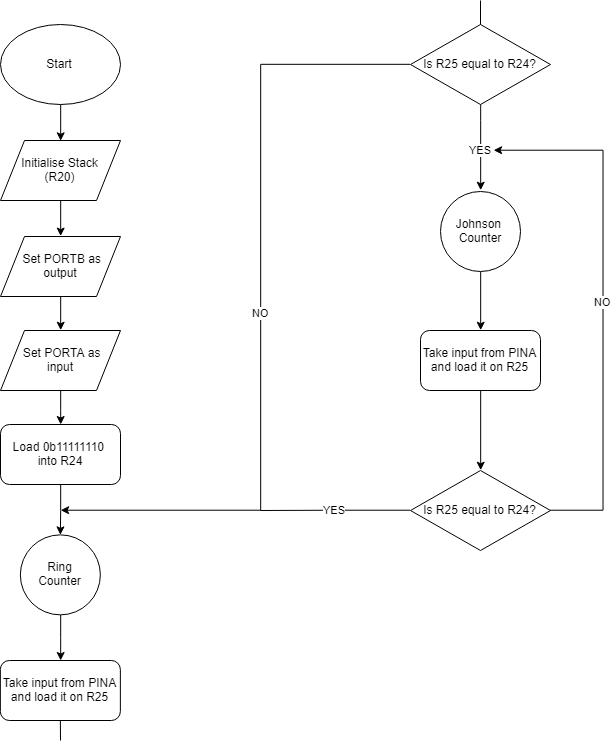
\includegraphics{img/Task1.png}
\end{center}


\section{Task 3}


\section{Task 4}


\section{Task 5}


\section{Task 6}



% Prints your bibliography database xxx.bib
\bibliographystyle{IEEEtran}
\bibliography{ref.bib}

\end{document}
